\documentclass[11pt]{article}
\usepackage[utf8]{inputenc}
\usepackage[spanish]{babel}
\usepackage[margin=2.2cm]{geometry}
\usepackage{graphicx}
\usepackage{longtable}
\usepackage{booktabs}
\usepackage{array}
\usepackage{hyperref}
\usepackage{enumitem}
\usepackage{titlesec}
\usepackage{xcolor}

\titleformat{\section}{\large\bfseries}{P\thesection.}{0.4em}{}
\renewcommand{\thesection}{\arabic{section}}

\begin{document}

% ============ CARÁTULA ============
\begin{titlepage}
\centering

{\large UNIVERSIDAD TÉCNICA ESTATAL DE QUEVEDO\par}
\vspace{0.1cm}
{\large FACULTAD DE CIENCIAS COMPUTACIONALES\par}
\vspace{0.1cm}
{\large CARRERA DE INGENIERÍA DE SOFTWARE, 4TO NIVEL\par}

\rule{\linewidth}{0.6pt}\par

{\Large\bfseries PRUEBA PRÁCTICA --- UNIDAD IV\par}
{\large Validación, Gestión, Herramientas y Estándares de Requisitos\par}
{\normalsize Caso: Sistema de Gestión de Pedidos\par}

\rule{\linewidth}{0.6pt}\par

\begin{tabular}{ll}
\textbf{Asignatura:} & Ingeniería de Requisitos (ISR-401) \\ [1pt]
\textbf{Estudiante:} & Alberto Jeanpool Marcillo Ponce \\ [1pt]
\textbf{Docente:} & Ing. Gleiston Guerrero Ulloa, PhD. \\
\end{tabular}

\vspace{0.10cm}

{\bfseries Repositorio:} \\
\url{https://github.com/amarcilloPoolgen/Marcillo-ISR401-Prueba-U4}

\vspace{0.3cm}

% ============ CAPTURAS ============
\centering
\fbox{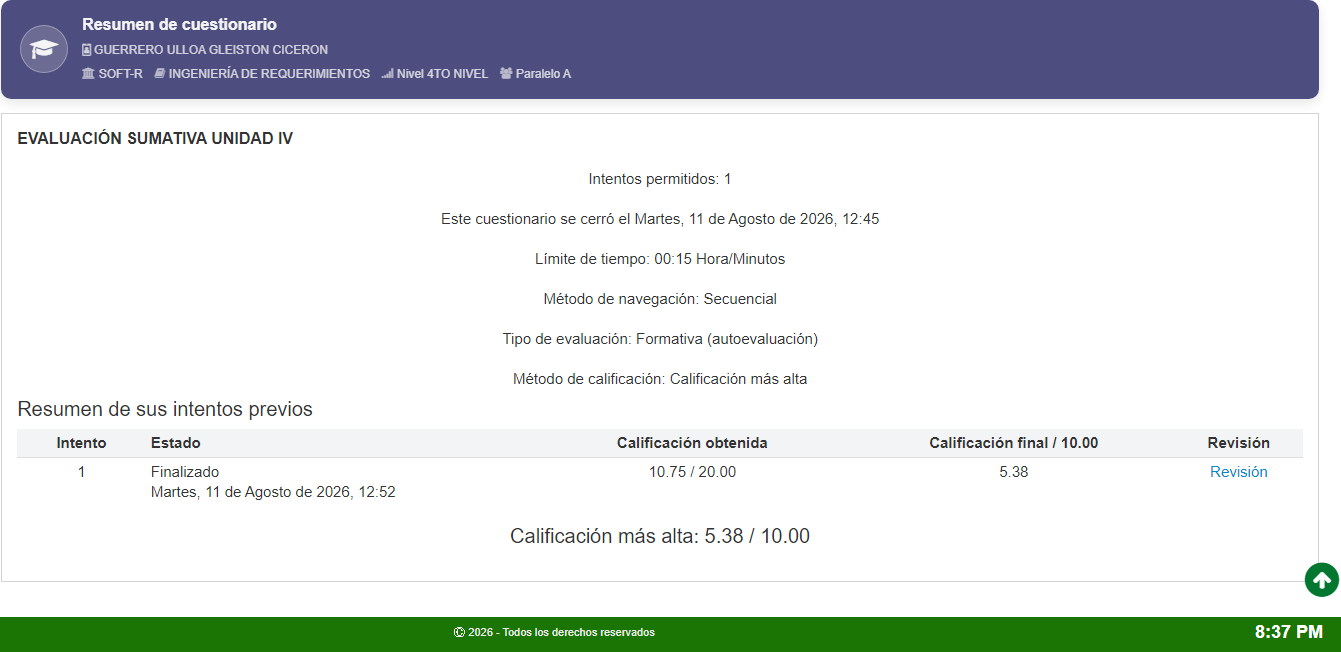
\includegraphics[width=0.8\textwidth,height=0.26\textheight,keepaspectratio]{captura_evaluacion.png}}\\[2pt]
{\small\itshape Fig. 1: Resumen del cuestionario}\\[10pt]
\fbox{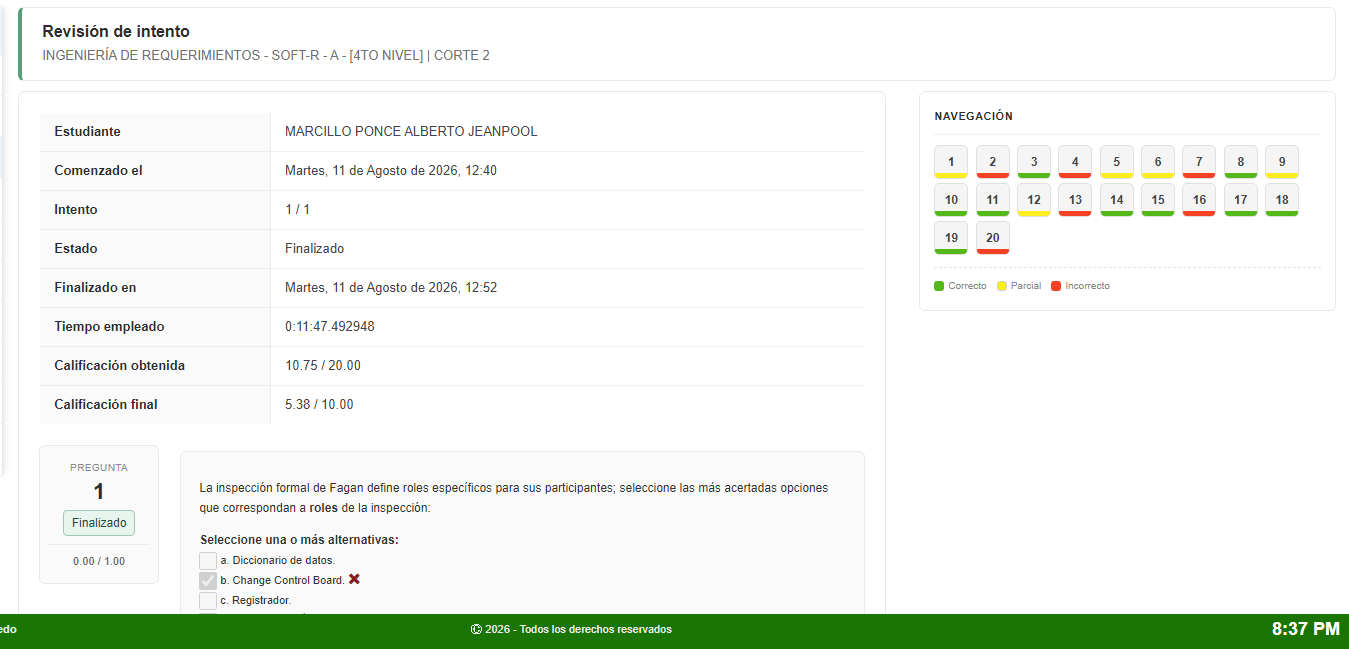
\includegraphics[width=0.8\textwidth,height=0.26\textheight,keepaspectratio]{captura_resumen.png}}\\[2pt]
{\small\itshape Fig. 2: Resultado de la evaluación (revisión de intento)}

\vspace{0.5cm}
{\normalsize Quevedo -- Ecuador\par}
{\normalsize \the\year\par}

\end{titlepage}

% ============ FIN CARÁTULA ============

{\centering\Large\bfseries Sistema de Gestión de Pedidos --- Respuestas (P1--P10)\par}
\vspace{0.3cm}

\section{Modelo de datos --- Diagrama de clases UML}

\begin{center}
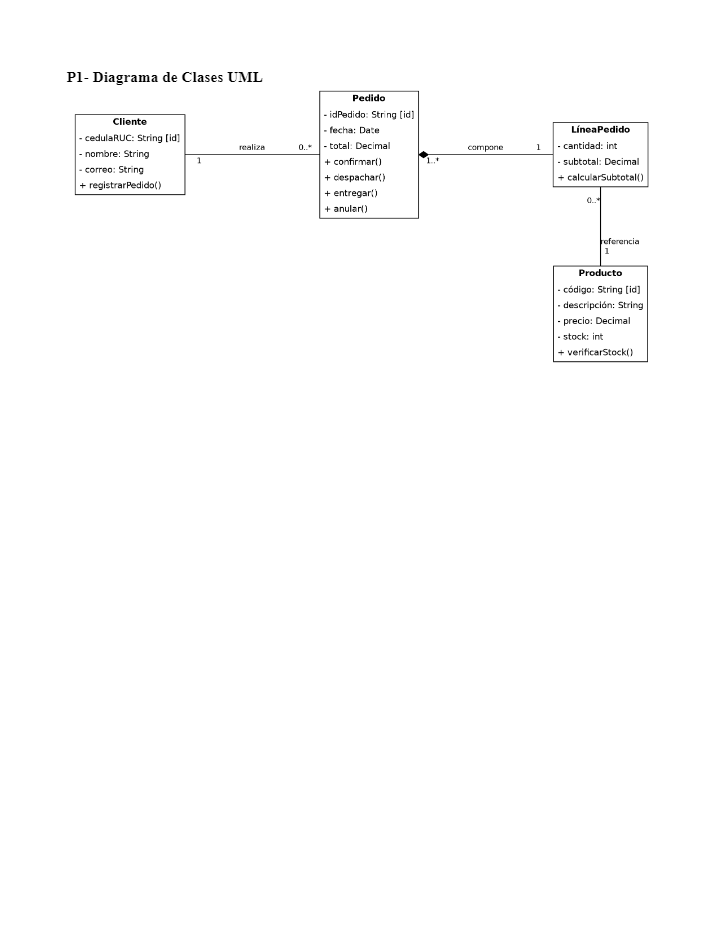
\includegraphics[width=0.95\textwidth]{p1_diagrama.png}
\end{center}

\textbf{Asociaciones y multiplicidades:}
\begin{itemize}[itemsep=1pt]
  \item Cliente 1 --- 0..* Pedido
  \item Pedido 1 --- 1..* LíneaPedido (composición)
  \item LíneaPedido 0..* --- 1 Producto
\end{itemize}

\section{Modelo funcional --- Diagrama de actividades ``Registrar pedido''}

\begin{center}
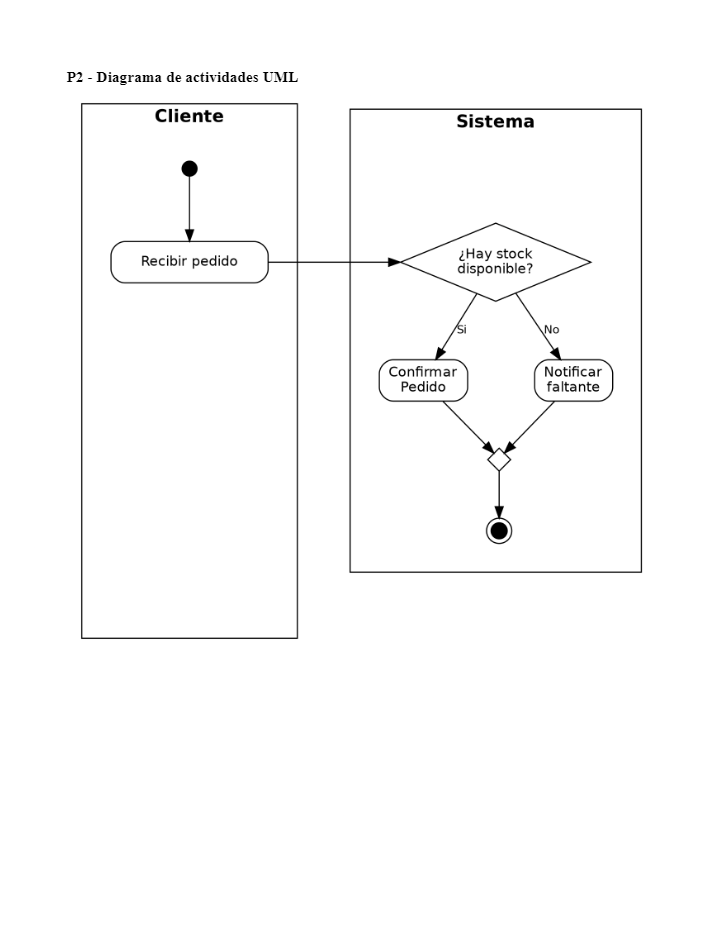
\includegraphics[width=0.75\textwidth]{p2_diagrama.png}
\end{center}

Inicio $\rightarrow$ Recibir pedido $\rightarrow$ Verificar stock (nodo de decisión) $\rightarrow$ [Sí] Confirmar pedido $\rightarrow$ Fin $\mid$ [No] Notificar faltante $\rightarrow$ Fin. Ambos caminos convergen antes del nodo final.

\textbf{Carriles de responsabilidad:} Cliente / Sistema.

\section{Modelo de comportamiento --- Máquina de estados de Pedido}

\begin{center}
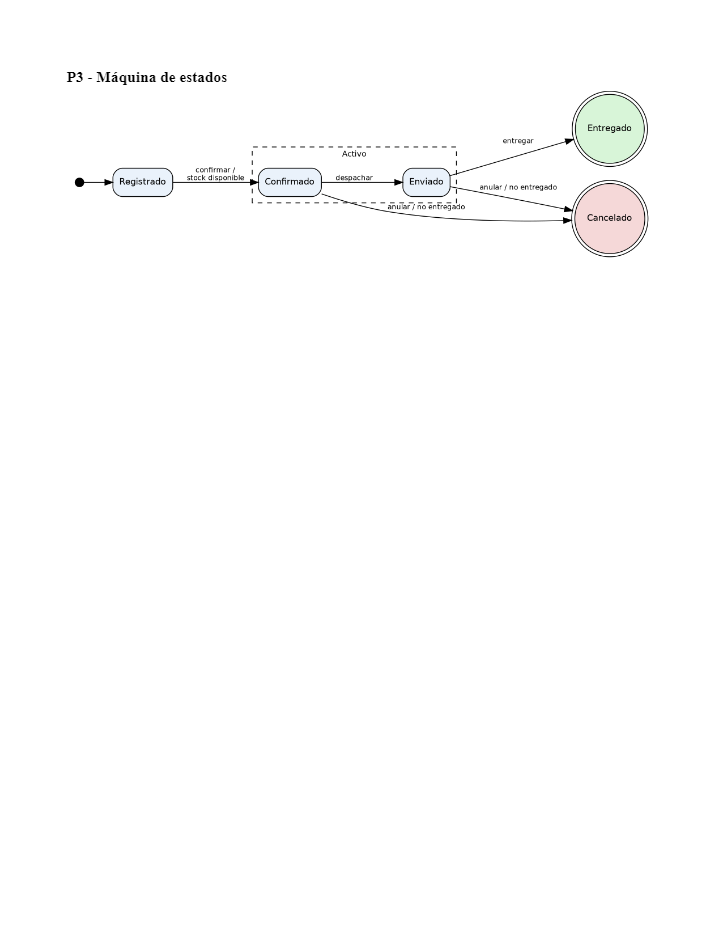
\includegraphics[width=0.95\textwidth]{p3_diagrama.png}
\end{center}

Registrado --[confirmar / stock disponible]$\rightarrow$ Confirmado --[despachar]$\rightarrow$ Enviado --[entregar]$\rightarrow$ Entregado (estado final).

Desde Confirmado o Enviado: --[anular / no entregado]$\rightarrow$ Cancelado (estado final).

\textbf{Superestado:} ``Activo'' agrupa \{Confirmado, Enviado\} con una transición de salida ``anular'' común, factorizando la transición hacia Cancelado.

\section{Consistencia entre las tres perspectivas}

\begin{center}
\small
\begin{tabular}{p{3.2cm}p{5cm}p{4.5cm}}
\toprule
\textbf{Evento (P3)} & \textbf{Función/Acción (P2)} & \textbf{Entidad/Atributo (P1)} \\
\midrule
confirmar & Confirmar pedido & Pedido.estado \\
despachar & Despachar pedido & Pedido.estado \\
entregar & Entregar pedido & Pedido.estado \\
anular & Anular pedido & Pedido.estado \\
\bottomrule
\end{tabular}
\end{center}

\textbf{Inconsistencia detectada:} el evento ``notificar faltante'' (P2) no tiene transición correspondiente en P3, ya que el pedido permanece en estado Registrado.

\textbf{Corrección:} se documenta como nota en la máquina de estados que dicho camino no produce cambio de estado (auto-transición interna en Registrado).

\section{Especificación de requisitos con esquema de atributos}

RF-01: El sistema debe permitir registrar un pedido con sus líneas y calcular el total automáticamente.

RF-02: El sistema debe verificar el stock del producto antes de confirmar el pedido.

RNF-01 (Eficiencia de desempeño, ISO/IEC 25010): el sistema debe registrar un pedido en menos de 3 segundos bajo carga normal.

RNF-02 (Seguridad, ISO/IEC 25010): los datos personales del cliente deben cifrarse en reposo y en tránsito.

\begin{center}
\small
\begin{tabular}{p{1.1cm}p{1.1cm}p{1.6cm}p{2.3cm}p{1.4cm}p{0.9cm}p{2.6cm}}
\toprule
\textbf{ID} & \textbf{Prior.} & \textbf{Estado} & \textbf{Fuente} & \textbf{Estabil.} & \textbf{Vers.} & \textbf{Verificación} \\
\midrule
RF-01 & Alta & Propuesto & Caso de\newline negocio & Alta & 1.0 & Prueba \\
RF-02 & Alta & Propuesto & Caso de\newline negocio & Alta & 1.0 & Prueba \\
RNF-01 & Media & Propuesto & Caso de\newline negocio & Media & 1.0 & Prueba de carga \\
RNF-02 & Media & Propuesto & Caso de\newline negocio & Media & 1.0 & Inspección/\newline prueba \\
\bottomrule
\end{tabular}
\end{center}

\section{Priorización MoSCoW}

\begin{itemize}[itemsep=2pt]
  \item \textbf{RF-01 --- Must have:} es el núcleo funcional del sistema.
  \item \textbf{RF-02 --- Must have:} garantiza integridad de datos e inventario.
  \item \textbf{RNF-01 --- Should have:} mejora la experiencia, pero no bloquea la operación básica.
  \item \textbf{RNF-02 --- Could have:} deseable desde el inicio, puede incorporarse en una iteración posterior.
\end{itemize}

\section{Validación por inspección (checklist ISO/IEC/IEEE 29148)}

\textbf{Propiedades evaluadas:} no ambiguo, completo, singular, verificable, factible.

\textbf{Defecto detectado (sin corregir):} RNF-02 no especifica algoritmo ni umbral medible $\rightarrow$ incumple ``verificable''.

\textbf{Retrabajo (segundo paso):} ``Los datos personales deben cifrarse con AES-256 en reposo y TLS 1.3 en tránsito.''

\section{Pruebas de aceptación trazadas}

\begin{center}
\small
\begin{tabular}{p{1.1cm}p{2.2cm}p{3.6cm}p{3.6cm}p{1cm}}
\toprule
\textbf{ID} & \textbf{Tipo} & \textbf{Entradas} & \textbf{Criterio de éxito} & \textbf{Traza} \\
\midrule
PA-01 & Funcional & Pedido con 2 líneas válidas & Total calculado correctamente & RF-01 \\
PA-02 & Funcional & Producto sin stock & Sistema notifica faltante, no confirma & RF-02 \\
PA-03 & No funcional & 100 pedidos simultáneos & Cada registro $<3$s & RNF-01 \\
PA-04 & No funcional & Intento de acceso directo a BD & Datos ilegibles sin clave & RNF-02 \\
\bottomrule
\end{tabular}
\end{center}

\section{Matriz de trazabilidad}

\begin{center}
\scriptsize
\begin{tabular}{p{1.4cm}p{2.2cm}p{4.2cm}p{1.3cm}}
\toprule
\textbf{Requisito} & \textbf{Fuente (atrás)} & \textbf{Modelo asociado} & \textbf{Prueba (adelante)} \\
\midrule
RF-01 & Caso de negocio & P1: Pedido/LíneaPedido; P2: flujo completo & PA-01 \\
RF-02 & Caso de negocio & P1: Producto.stock; P2: decisión stock & PA-02 \\
RNF-01 & Caso de negocio & P2: flujo ``Registrar pedido'' & PA-03 \\
RNF-02 & Caso de negocio & P1: Cliente (datos personales) & PA-04 \\
\bottomrule
\end{tabular}
\end{center}

\textbf{Dependencia horizontal:} RF-02 depende de RF-01 (no puede verificarse stock sin un pedido creado).

\textbf{Requisitos huérfanos:} ninguno; los cuatro requisitos cuentan con modelo y prueba asociados.

\section{Gestión del cambio y línea base}

\textbf{Solicitud de cambio:} ``Agregar notificación por correo al cliente al confirmar el pedido''.

\textbf{Análisis de impacto (según matriz P9):} afecta a RF-01, al diagrama de clases (nuevo método en Pedido) y a la prueba PA-01.

\textbf{Decisión del CCB:} Aprobada, prioridad Should have. \quad \textbf{Nueva versión:} RF-01 pasa de v1.0 a v1.1.

\textbf{Línea base declarada (Baseline 1.0):} se congela la configuración coherente: ERS v1.0, modelos de clases/actividades/estados v1.0, matriz de trazabilidad v1.0 y pruebas de aceptación v1.0.

\end{document}
